\chapter{The Pressure Signature of Aeroacoustic Sources}
The genesis for this project first began with the work of Sinha \etal [cite], which studied the irrotational near-field response of a subsonic jet subjected to excitation with plasma actuators by decomposing the instantaneous fluctuating pressure field into a coherent `wave' component (which corresponds to the large-scale structure generated by the excitation) and incoherent residual fluctuations (which correspond to the natural turbulence in the jet). 
Fundamentally, this decomposition is similar to the triple decomposition used by Hussein \& Reynolds [cite].
Sinha \etal [cite] found that each pulse from the actuators produces a coherent large-scale structure that would grow, saturate, and decay as it advects through the jet shear layer. 

In the irrotational near-field, the signature of these large-scale structures takes the form of a compact waveform. 
At low enough excitation frequencies, the characteristic period of this waveform is much less than the excitation period, and hence, the structures seeded by the excitation do not interact with one another as they evolve downstream. 
Therefore, their behavior can be thought of as representing the response of the jet to a single perturbation; in short this is the `impulse' response of the jet, which is produced by the impulsive excitation by LAFPAs.
As the period of actuation approaches the characteristic period of the impulse response, the waveforms extracted by the phase-averaging technique are largely unmodified from that of the impulse response. 
Above this frequency, significant interaction between the structures is observed, with noticeable modifications to the waveform shape and amplitude. 
As the structures are growing as they advect through the shear layer, the frequency at which the structures begin to interact is dependent on the axial location.
This behavior can be observed in \fig{fig:ch3_nearfield_phavg}.
\begin{figure}
	\centering
	\begin{subfigure}{.5\textwidth}
		\centering
		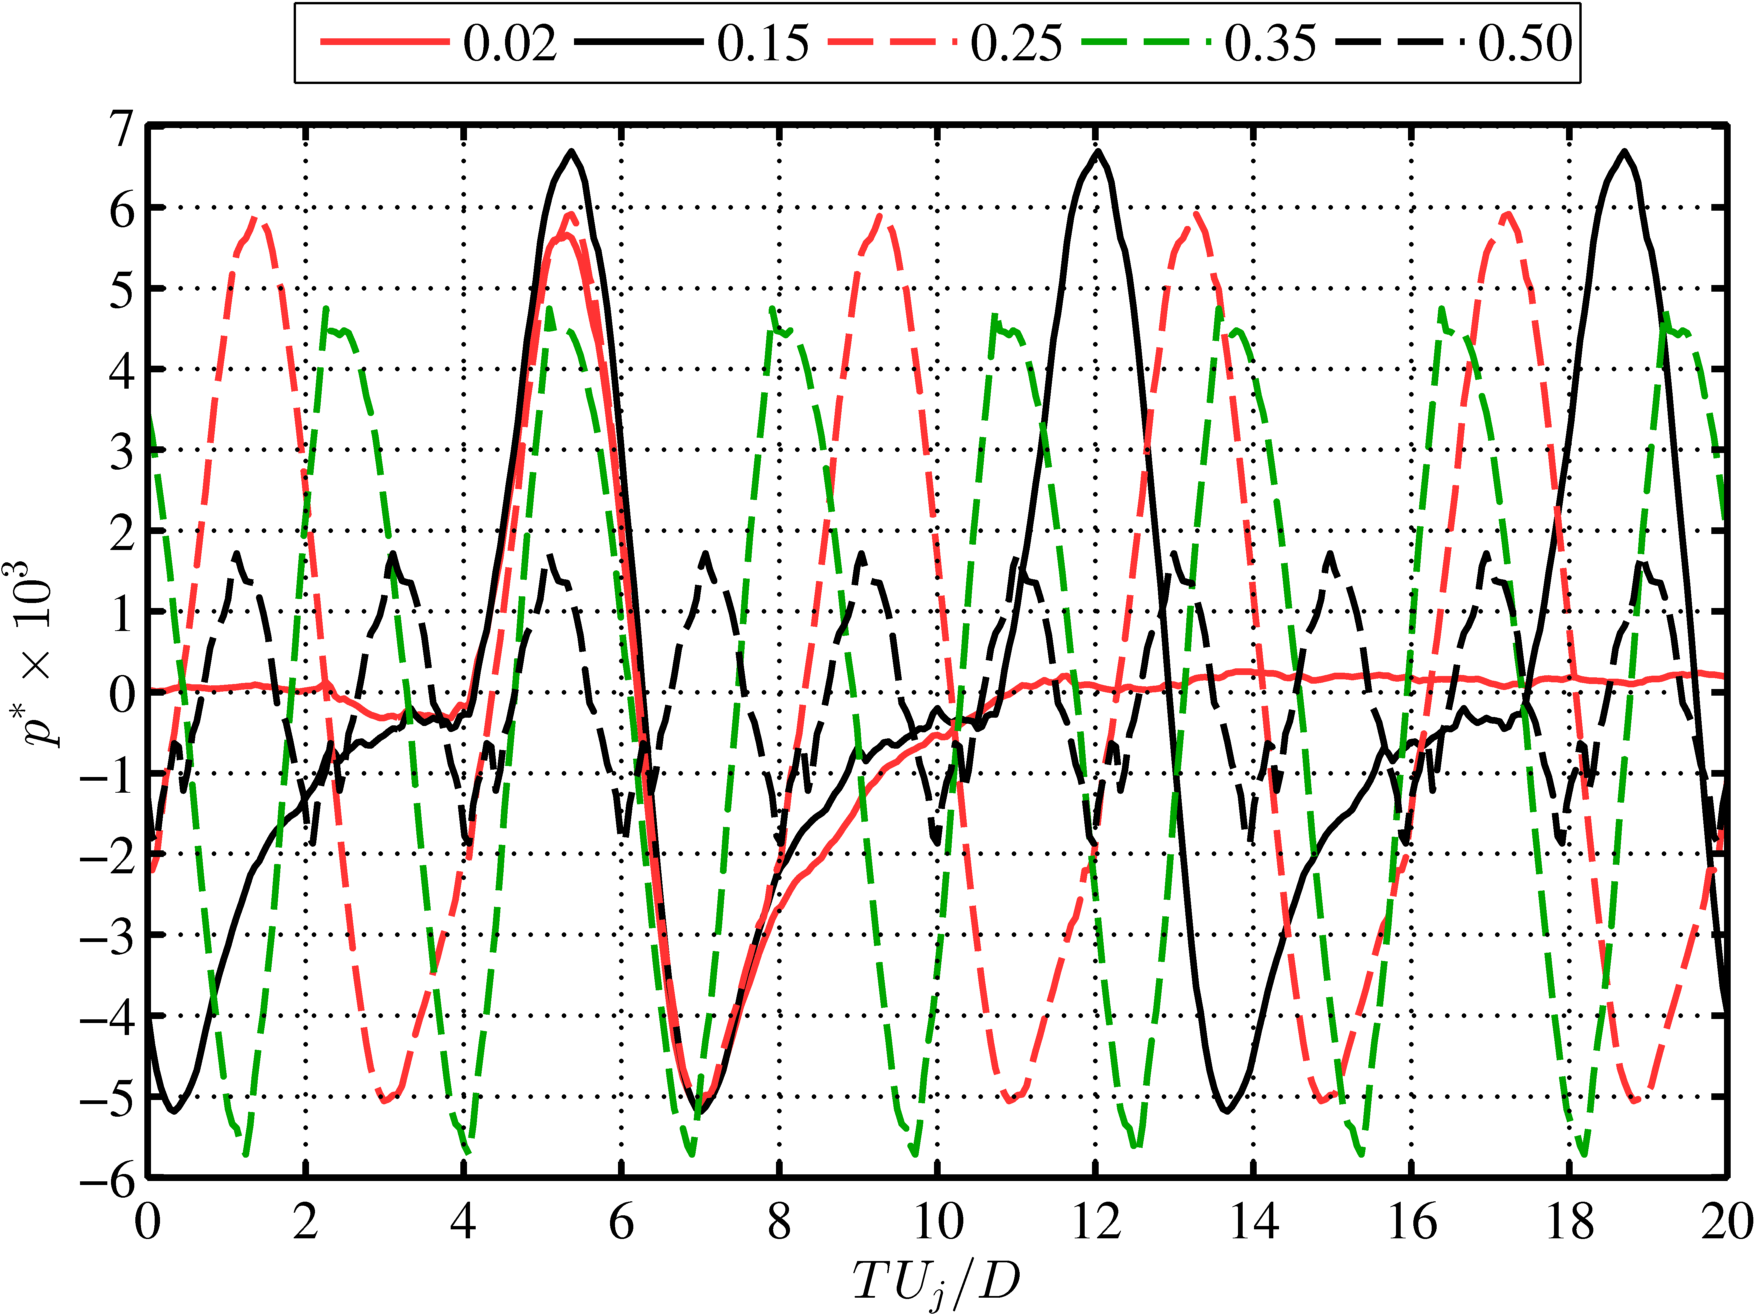
\includegraphics[width=0.95\linewidth]{Figures/ch3_nearfield_phavg.png}
		\caption{}
		\label{fig:ch3_nearfield_phavg}
	\end{subfigure}%
	\begin{subfigure}{.5\textwidth}
		\centering
		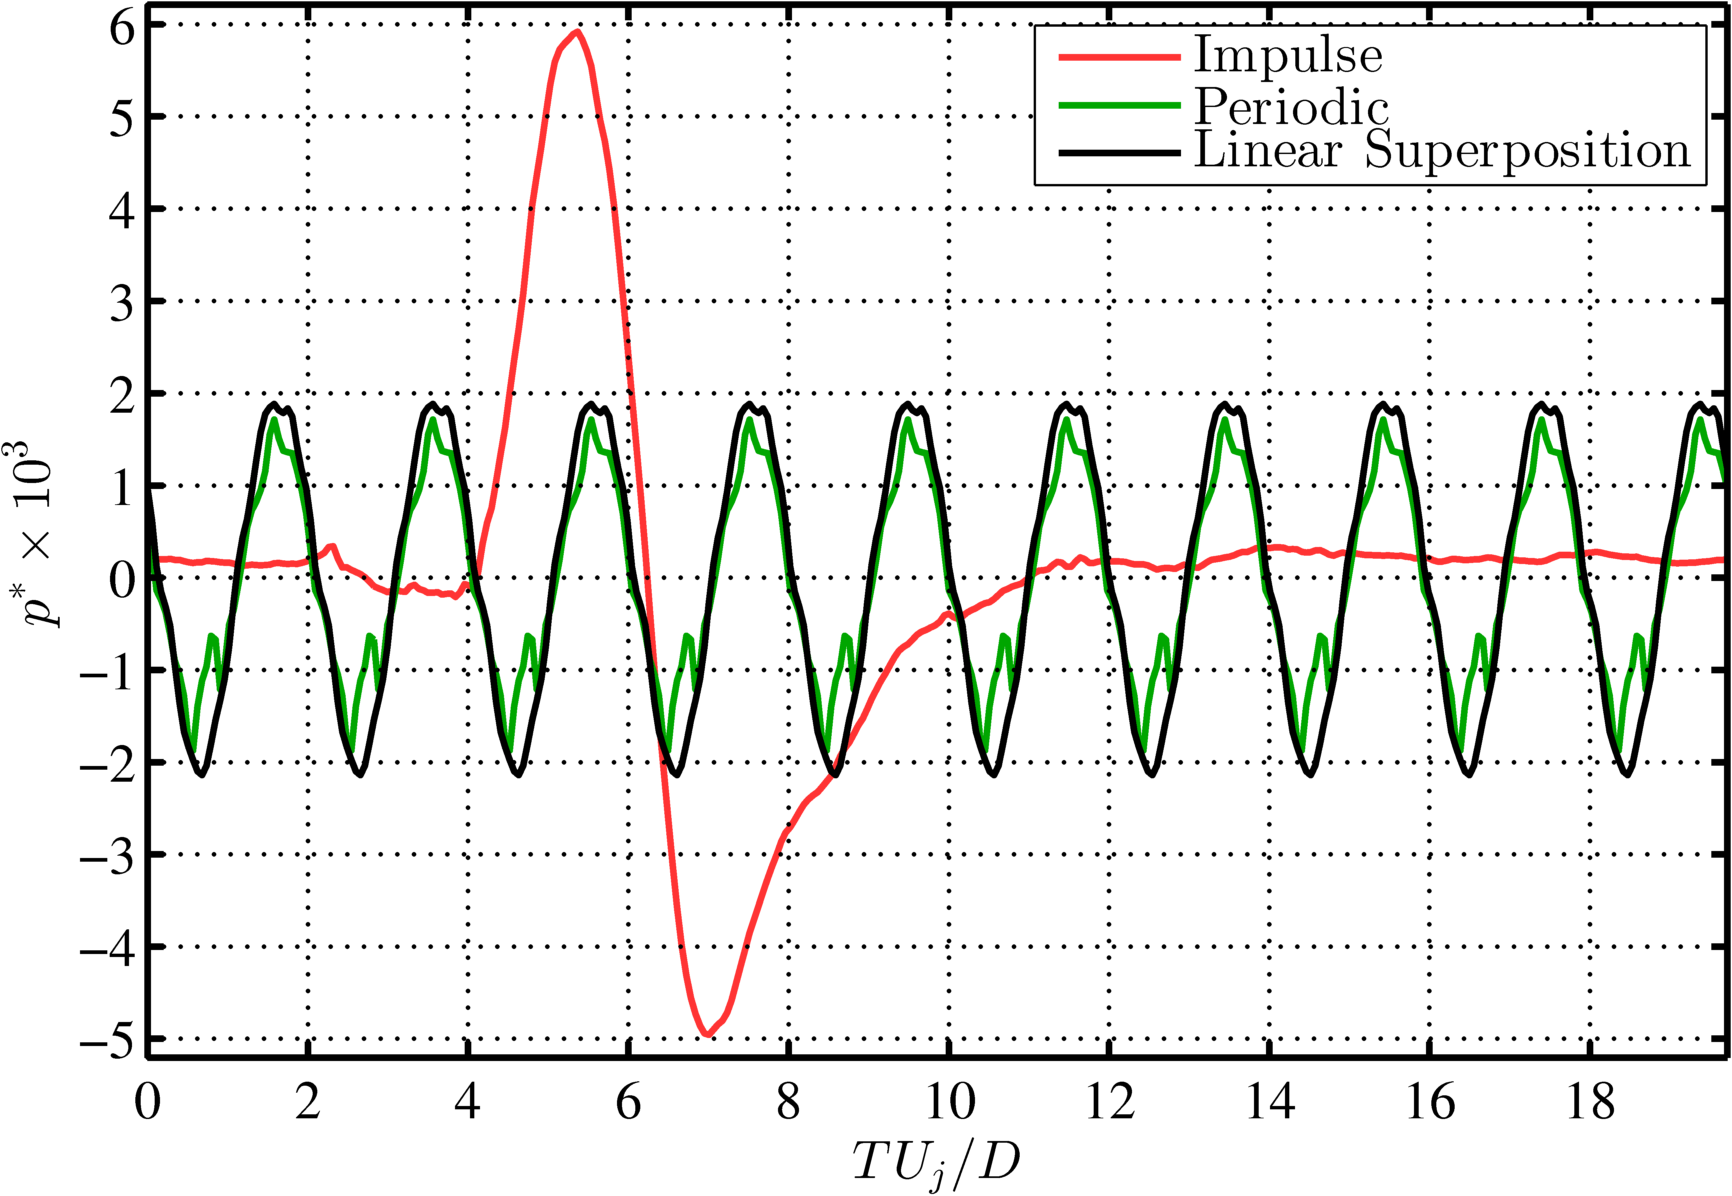
\includegraphics[width=0.95\linewidth]{Figures/ch3_nearfield_linear.png}
		\caption{}
		\label{fig:ch3_nearfield_linear}
	\end{subfigure}
	\caption{Phase-averaged waveforms along the first array position at $z/D = 3, r/D = 1.35$ (a) and a linear superposition of the phase-averaged waveform for the impulse excitation ($St_{DF} = 0.05$) compared against periodic excitation ($St_{DF} = 0.50$) (b).}
	\label{fig:ch3_nearfield}
\end{figure}

For a certain range of excitation frequencies ($St_{DF} \leq 0.50$ at $z/D = 2$, for example), the structures interact in a quasi-linear manner, insofar as their near-field pressure signatures are concerned. 
To be precise, the response of the jet in the irrotational near-field could be well-predicted by a linear summation of the impulse response of the jet, repeated at the periodic excitation frequency. 
This concept has been illustrated in \fig{fig:ch3_nearfield_linear}, where the periodic response of the jet to excitation with $St_{DF} = 0.50$ has been reproduced at $z/D = 3$ 8. 
Additionally, a linear superposition of the impulse response for $St_{DF} = 0.05$, repeated to match the excitation frequency of $St_{DF} = 0.50$, has been overlaid. 
The linear superposition has been arbitrarily shifted in time in order to match the phase of the periodic response; this phase difference is likely due to the dependence of convection velocities on structure frequency [Veltin] (or more accurately, structure size). 
For reference, the impulse response has also been included in the plots. 
Upstream of the end of the potential core ($z/D = 6$, as determined previously in our facility by PIV [Kearney]), the quasi-linear interaction model produces close predictions of the waveform amplitude and shape, despite the significant difference in both peak amplitude and waveform shape between the impulse and periodic responses. 

\section{Preprocessing: Filtering the Actuator Self-Noise}
Analysis of the near-field response of the forced jet is not immediately straightforward due to acoustic contamination from the actuators themselves [Kearney]. 
LAFPAs operate on a joule heating principle: the breakdown of the air between the electrodes and the ensuing flow of current results in intense heating of the air. This rapid, localized thermal perturbation produces a compression wave, which excites the shear layer. 
However, this compression wave is still evident as it travels through the near field. 
Multiple compression waves can clearly be seen in \fig{fig:self-noise}, in which a subsonic rectangular jet is being excited at 20 kHz by four LAFPAs on its lower edge. \begin{figure}
	\centering
	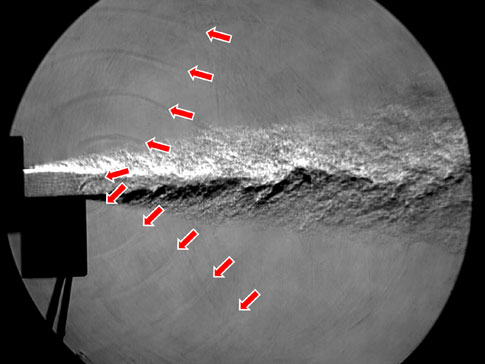
\includegraphics{Figures/Samimy2010JFM.jpg}
	\caption{Schlieren image highlighting LAFPA compression waves. Reprinted from Samimy 2010 JFM.}
	\label{fig:self-noise}
\end{figure}

Obviously, this is an undesirable effect, as this actuator self-noise may in some cases obscure the hydrodynamic and acoustic response of the jet.
So, in the present work the near-field pressure signals have been preprocessed using a continuous-wavelet-based filtering algorithm, which has been specifically designed to remove the actuator self-noise while leaving the signature of the jet response unaltered. 
An example of this filtering can be found in \fig{fig:preprocessing:wavelet_filter}, where the raw and preprocessed signals have been plotted for $St_{DF} = 0.02$ at $x/D = 1$, $r/D = 1.20$. 
To aid in visualization, the results for multiple excitation periods has been phase-averaged to produce these waveforms. 
As the actuator self-noise is localized in both time and frequency and can be well predicted, a smoothing algorithm in the wavelet domain was found to be the most effective method for removing the undesirable noise while leaving the response of the jet intact. 
A fourth-order Paul wavelet is employed, due to the similarity of its imaginary component to the phase-averaged response of the jet. 
As a result, the energy of the response of the jet is well defined in the wavelet domain, with the actuator self-noise existing as high-frequency, temporally-localized oscillations superimposed on the field. 
After smoothing in the wavelet domain to remove these oscillations, the signal is transformed back into the physical domain where it undergoes another smoothing operation in order to remove small amplitude, high frequency oscillations which may be introduced by the wavelet-smoothing. 
For consistency hereafter, all results examined within this work have been computed from the filtered, rather than the raw, signals.
\begin{figure}
	\centering
	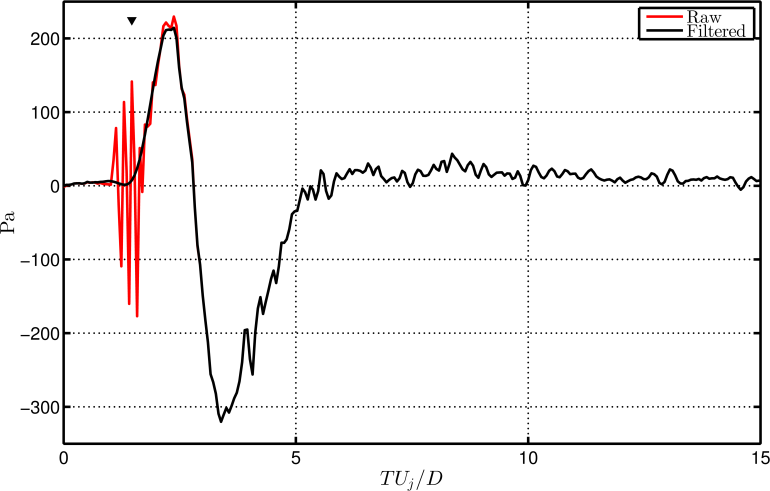
\includegraphics{Figures/NearField_Preprocessing_Filtering.png}
	\caption{Raw and preprocessed near-field pressure.}
	\label{fig:preprocessing:wavelet_filter}
\end{figure} 

\section{Far-field Response}
\section{Acoustic/Hydrodynamic Decomposition}
Much of the difficulty in identifying the aeroacoustic source terms revolves around the dissimilar range of scales and fluctuation intensities of the turbulent eddies in the shear layer and the resulting radiated noise. 
Outside the jet shear layer, in the irrotational near-field of the jet, strong hydrodynamic pressure fluctuations associated directly with the passage of coherent structures in the shear layer and their resultant weak acoustic radiation coexist [Arndt]. 
Beyond this, in the acoustic far-field, the hydrodynamic signature of the coherent structures is nonexistent owing to their strong exponential decay with radial distance.
It is in the irrotational near-field that much work has focused, in order to improve the aeroacoustic community's understanding of the link between shear layer turbulence and far-field acoustic radiation. 

Owing to the presence of strong hydrodynamic fluctuations dominating the irrotational pressure field near the noise source regions, identification of pure acoustic waves and their corresponding source events is problematic.
A decomposition of the pressure field into its constitutive hydrodynamic and acoustic components is therefore required. 
By identification and prediction of coherence nulls in the near field, Coiffet \etal [cite] showed that the full irrotational near-field consistent primarily as a linear superposition of its hydrodynamic and acoustic components, which lead subsequent researchers to propose linear filters to extract the individual components from the near-field pressure, with varying degrees of success. 

As discussed by Tinney \& Jordan [cite], in a transonic jet in which the large-scale structures are convecting subsonically with respect to the ambient speed of sound, a demarcation of the hydrodynamic and acoustic energy fields can be observed with phase velocity.
This is because the hydrodynamic pressure fluctuations will be aligned with the jet axis, and travelling subsonically. 
Acoustic pressure fluctuations will impinge on the linear microphone array at oblique angles, and therefore will appear as having either sonic or supersonic phase velocity, based on the source location. 
Therefore, a demarcaction between the hydrodynamic and acoustic energy components should be readily identifiable about the sonic wavenumber, $k_a = \omega / a_\infty$.

An illustration of this can be found in \fig{fig:phase_velocity_map}, where the power spectral density of the irrotational near-field pressure for a single microphone array position has been plotted as a function of normalized frequency and (axial) wavenumber.
The sonic velocity has been identified with a dashed line; energies lying above this line correspond to supersonically traveling waves (and hence, acoustic energy) whereas energies below this line correspond to subsonically convecting waves (hydrodynamic energy).
Note that at high wavenumber and frequencies, two distinct energy lobes become readily apparent.

This phase-velocity separation is the basis for the decomposition method of Tinney \& Jordan [cite], which used a Fourier-based wavenumber-frequency filter in a cold, subsonic jet to separate the near-field pressure into supersonically- and subsonically-convecting waves.
The pressure field is first transformed into Fourier space ($k_x,\omega$), as
\begin{equation}
	\hat{p} \left( k_x , \omega \right) = \iint_{\mathbb{R}^2} p(x,t)e^{-i(\omega t - k_x x)}dxdt
\end{equation}
From the transformed pressure field, the hydrodynamic and acoustic fields can then be reconstructed separately, from
\begin{equation}
	p_c (x,t) = \frac{1}{(2 \pi)^2} \iint_{\mathbb{R}^2} \phi_c (k_x,\omega) \hat{p} (k_x,\omega)e^{i(\omega t - k_x x)}dk_x d\omega .
	\label{eq:fourier_filter}
\end{equation}
The component weight vector, $\phi_c \in [0,1]$, is set based on the measured axial phase velocity, $c = \omega / k_x$ in order to filter out either the supersonic or subsonic portion of the spectra. 
 
Grizzi \& Camussi [cite] took a slightly different approach, which utilized a discrete wavelet transform at individual spatial locations in order to decompose the fields based on an energy cutoff. 
The energy threshold was set iteratively, using analysis of two-point correlations of the acoustic and hydrodynamic components between two microphones, in order to ensure that realistic phase-velocities for the components were met. 
The Empirical Mode Decomposition (EMD) based method of Kuo \etal [cite] dispensed with explicit concerns with the phase velocity of the pressure components and instead used the critical frequency, as defined by Arndt \etal [cite], which demarcates the energy dominance of the acoustic and hydrodynamic components in the near-field spectra.
[Include recent Yonglu paper?]
\begin{figure}
	\centering
	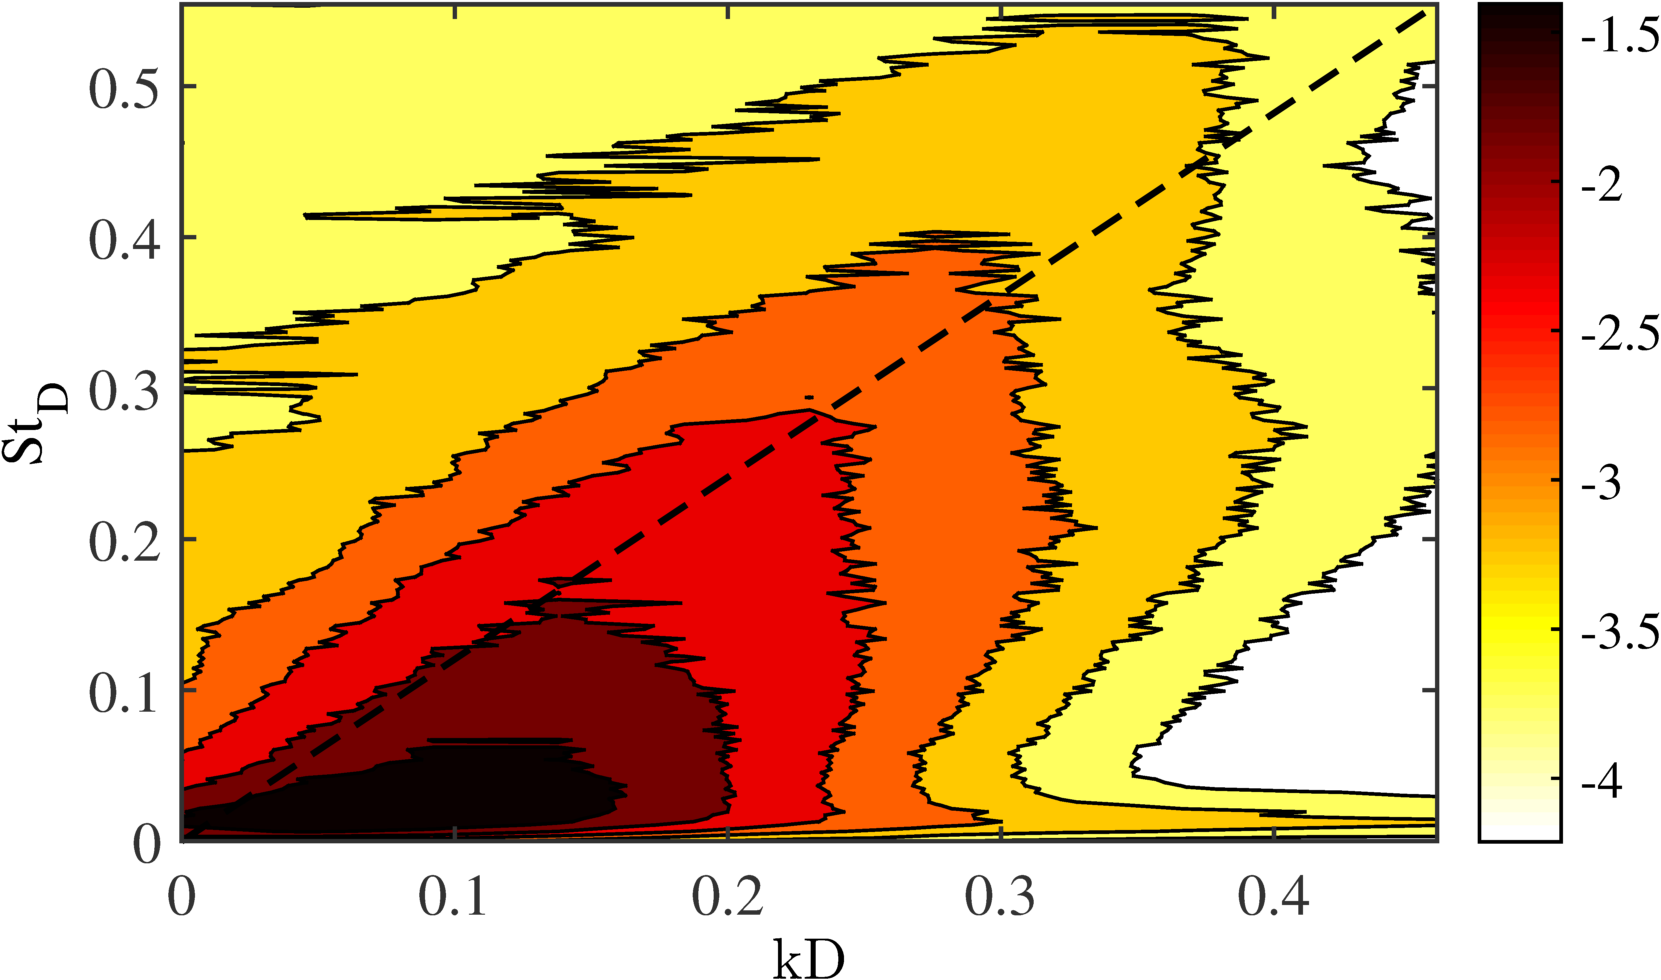
\includegraphics[width=4in]{Figures/Phase_Velocity_Map.png}
	\caption{Wavenumber-Frequency spectral energy.}
	\label{fig:phase_velocity_map}
\end{figure}

In the current work, the irrotational near-field pressure is decomposed into its constitutive hydrodynamic and acoustic components based on phase-velocity. 
The current method is similar to that of Tinney \& Jordan [cite] in that an axial array of many microphones is used, though it differs in how it identifies components of different phase-velocity.
Here, the filtering will be performed by a spatio-temporal continuous wavelet transform.

\subsection{The Wavelet Transform}
Fourier analysis is commonly employed in the aeroacoustics community to study fundamental aspects of jet noise due to its simplicity and the great abundance of information it can provide. 
However, there is also a great drawback associated with Fourier analysis: while it analyzes a given signal at a distinct frequency, local information for a given event is spread over all spectral coefficients. 
This is due to the fact that the basis functions used by the Fourier transform oscillate indefinitely. 
For a completely stationary signal this is not an issue, however it has become increasingly clear that the jet noise phenomenon is not a stationary process.
Transient events, such as intermittency or the spatial and temporal modulation of a wavepacket, have been shown to be important in the noise generation process. 

Grossman [cite] introduced the wavelet transform in an effort to overcome some of the shortcomings of the Fourier transform.
Unlike the Fourier transform, the wavelet transform involves a convolution of the signal with a set of basis functions which decay to zero at the bounds.
As a direct result, translation of the basis function in space and/or time is now meaningful. 
The basis functions (often referred to as the analyzing or daughter wavelets) are all derived from a single function, the mother wavelet, which must satisfy certain criteria [Farge],
Most notable of of these criteria is that of admissibility, which in essence requires that the wavelet must be of finite energy. 
In practice, it is also helpful to choose a mother wavelet which is well-localized in both the spatio-temporal domain and the frequency domain. 
For a given mother wavelet, $\psi (\vec{x})$, the daughter wavelets can be constructed as
\begin{equation}
	\psi_d \left( \vec{x};s,\vec{\tau},\theta \right) = s^{-n/2} \psi \left( s^{-1} r_{-\theta} \left(\vec{x}-\vec{\tau} \right) \right) \
	\label{eq:daughter_wavelets}
\end{equation}
where $s$ is the scale factor, $\vec{\tau}$ the translation parameter, and in the case of a multidimensional transform, $r_{-\theta}$ is the rotation vector (which can be neglected for an isotropic mother wavelet). 
The $s^{-n/2}$ factor ensures constant energy across all dilations. 
For a specific scale, translation, and rotation, the wavelet transform then becomes
\begin{equation}
	\tilde{f} \left( s, \vec{\tau}, \theta \right) = \int_{\mathbb{R}^n} f \left( \vec{x} \right) \psi^*_d \left( \vec{x};s,\vec{\tau},\theta \right) d^n \vec{x}.
\end{equation}

Because the basis functions of the wavelet transform are of finite energy, the locality of information in the original signal is preserved in the wavelet coefficients. 
This allows the identification, analysis, and reconstruction of localized events in the original signal, something not possible with the Fourier transform, which spreads temporal/spatial information over all transform coefficients. 
This has enabled previous researchers to perform a range of new analysis techniques to turbulence and acoustic phenomena not possible with the traditional Fourier transform. An excellent review of the development of wavelet analysis as well as applications to turbulence can be found in Farge [cite].

Use of a multidimensional, continuous wavelet transform to extract intermittent events with a specific phase-velocity is not immediately straightforward, due to the global nature of the scale factor. 
A `speed-tuning' parameter, $c$, was introduced to the wavelet transform (now specifically referred to as a \textit{spatio-temporal} wavelet transform) by Antoine \etal [cite], who used it for use in motion tracking and identification in two-dimensional images. 
The definition for the daughter wavelets (\ref{eq:daughter_wavelets}) is modified to
\begin{equation}
	\psi_d \left( \vec{x}, t;s,\vec{x}', t' \right) = s^{-n/2} \psi \left(s^{-1} c^{-1/n} (\vec{x}-\vec{x}'), s^{-1} c^{(n-1)/n} (t-t') \right)
\end{equation} 
where $n$ corresponds to the total number of dimensions (temporal and spatial).

The continuous wavelet transform are isometry [Antoine] and hence is invertible.
The original signal may therefore be recovered from the wavelet coefficients as 
\begin{equation}
	f(\vec{x},t) = \frac{1}{C_\delta} \int_0^\infty \frac{ds}{s^{1 + n/2}} \int_{0}^{\infty} \frac{dc}{c} \tilde{f} (\vec{x},t,s,c).
	\label{eq:wavelet_filter}
\end{equation}

The constant factor $C_\delta$ serves as an energy scaling, and appears because we are reconstructing the signal using a different analyzing wavelet (in this case, a delta function) than the mother wavelet used in the forward transform [Torrence,Farge,Antoine]. 
For a given mother wavelet, this factor can be found from
\begin{equation}
	C_\delta = \frac{1}{(2 \pi)^n} \int_0^\infty \frac{ds}{s^{1 + n/2}} \int_{0}^{\infty} \frac{dc}{c} \int_{\mathbb{R}^{n-1}} d \vec{k} \int_{-\infty}^{\infty} d\omega \hat{\psi}_d^*
\end{equation}
where $\hat{\psi}_d$ are the daughter wavelets in Fourier space. 
Since we are interested in decomposing the field into the acoustic and hydrodynamic components, a filtered reconstruction can be done quite easily in the wavelet domain by simply modifying the integration limits in \eq{eq:wavelet_filter} to include only speed-tuning parameters corresponding to the subsonic or supersonic portion of the wavelet spectrum.

In this way, this methodology can be thought of as a simple modification of that proposed by Tinney \& Jordan [cite], replacing the Fourier transform in their method with a spatio-temporal wavelet transform. 
The relationship between the wavelet transform and the Fourier transform can be further elucidated by computing the forward transform in the Fourier domain (with the use of the convolution theorem), inserting this into \eq{eq:wavelet_filter}, and reversing the order of the integration:
\begin{multline}
		f_c (\vec{x},t) = \frac{1}{(2 \pi)^n} \int_{\mathbb{R}^{n-1}} d \vec{k} \int_{-\infty}^{\infty} d\omega \hat{f}(\vec{k},\omega) e^{i(\omega t - \vec{k} \cdot \vec{x})} \\ 
		\times \frac{1}{C_\delta} \int_0^\infty \frac{ds}{s^{1 + n/2}} \int_{0}^{\infty} \frac{dc}{c} \hat{\psi}_d^* (sc^{1/2}k,sc^{-1/2} \omega)
\end{multline}
\begin{equation}
	f_c (\vec{x},t) = \frac{1}{(2 \pi)^n} \int_{\mathbb{R}^{n-1}} d \vec{k} \int_{-\infty}^{\infty} d\omega \hat{f}(\vec{k},\omega) e^{i(\omega t - \vec{k} \cdot \vec{x})} \phi_c (k,\omega)
	\label{eq:wavelet_filter_simplified}
\end{equation}
The appearance of \eq{eq:wavelet_filter_simplified} is identical to that of \eq{eq:fourier_filter}; the difference lies in how filter $\phi_c$ is defined, either explicitly in the Fourier domain in the case of the Fourier filtering or implicitly by the shape of the chosen mother wavelet in the wavelet transform. 
As numerous other researchers have discussed, this leads to an alternative interpretation of the wavelet transform, that of a series of bandpass filters, the passband envelope, centroid, and width being dictated by the scale, speed, and mother wavelet [Farge, torrence].

In fact, computing the convolutions is much faster in the Fourier domain than in the physical domain, so \eq{eq:wavelet_filter_simplified} is the preferred method for computing the spatio-temporal wavelet filter.
The decompositions were performed along each radial microphone array position individually, using the (1+1) dimensional (space-time) Morlet wavelet as the mother wavelet:
\begin{equation}
	\psi (x,t) = e^{i(k_o x + \omega_0 t)} e^{-(x^2 + t^2)/2}
\end{equation}
which the reader will recognize as simply a plane wave modulated by a Gaussian. 
Though simplicity was a factor in this decision, previous results analyzing phase-averaged waveforms in the far-field found acoustic emissions with a characteristic waveform that share some resemblance to the Morlet wavelet [crawley2014]. 
The base oscillation frequencies, 〖$(k_0,\omega_0)$ were set to $(\pm 5,5)$ (the dual sign for $k_0$ being necessary to recover both forward and backward traveling waves), and $\hat{\psi}(k,0) = 0$ and $\hat{\psi}(0,\omega) = 0$ so as to ensure that the mother wavelet met the admissibility criterion.

As the microphone array is irregularly spaced in the axial direction, the pressure field was interpolated onto a regular grid of spacing $1D$ before computation of the discrete Fourier transform. 
In the current work, the local speed of sound was chosen as the phase-velocity demarcation, as opposed to the ambient speed of sound which had been used by previous researchers [Tinney and Jordan]. 
In our case, the jet under study is subsonic and unheated, meaning that the local speed of sound (~320 m/s) is still greater than the jet velocity (~287 m/s) yet lower than the ambient speed of sound (~346 m/s) and hence is a better choice for this particular application.
\subsection{Validation}
Though broad in its view, a simple evaluation of the decomposition algorithm can first be made by examination of the radial decay of the pressure fluctuation intensities, as has been done in \fig{fig:ch3_validation_Pms}  at an axial position near the end of the potential core. 
Theoretical analysis by Ribner [cite] and Arndt \etal [cite] showed that the intensity of the full hydrodynamic field (as opposed to the inertial field alone) decays as $I \sim r^{-6}$. 
In contrast, the acoustic field has been shown to be well-approximated by the linearized Euler equations, which exhibit $I \sim r^{-2}$ decay rates (that is, the field is dominated by spherically propagating waves). 
Hence, the individually processed microphone array positions can serve as an initial validation step for the radial decay of the decomposed fields.

Comparison of the theoretical and measured radial decay rates for the decomposed acoustic and hydrodynamic fields can be found in \fig{fig:ch3_validation_Pms}.
Overall, good agreement is found between the decomposed fields and the expected radial decay rates, indicating that on a broad level the decomposition algorithm is identifying and extracting the individual acoustic and hydrodynamic fields irrespective of the relative amplitudes of the two fields.
However, it is observed that the decomposition produces an acoustic field which decays at a rate which is slightly slower than that dictated by spherically-spreading sound waves. 
\begin{figure}
	\centering
	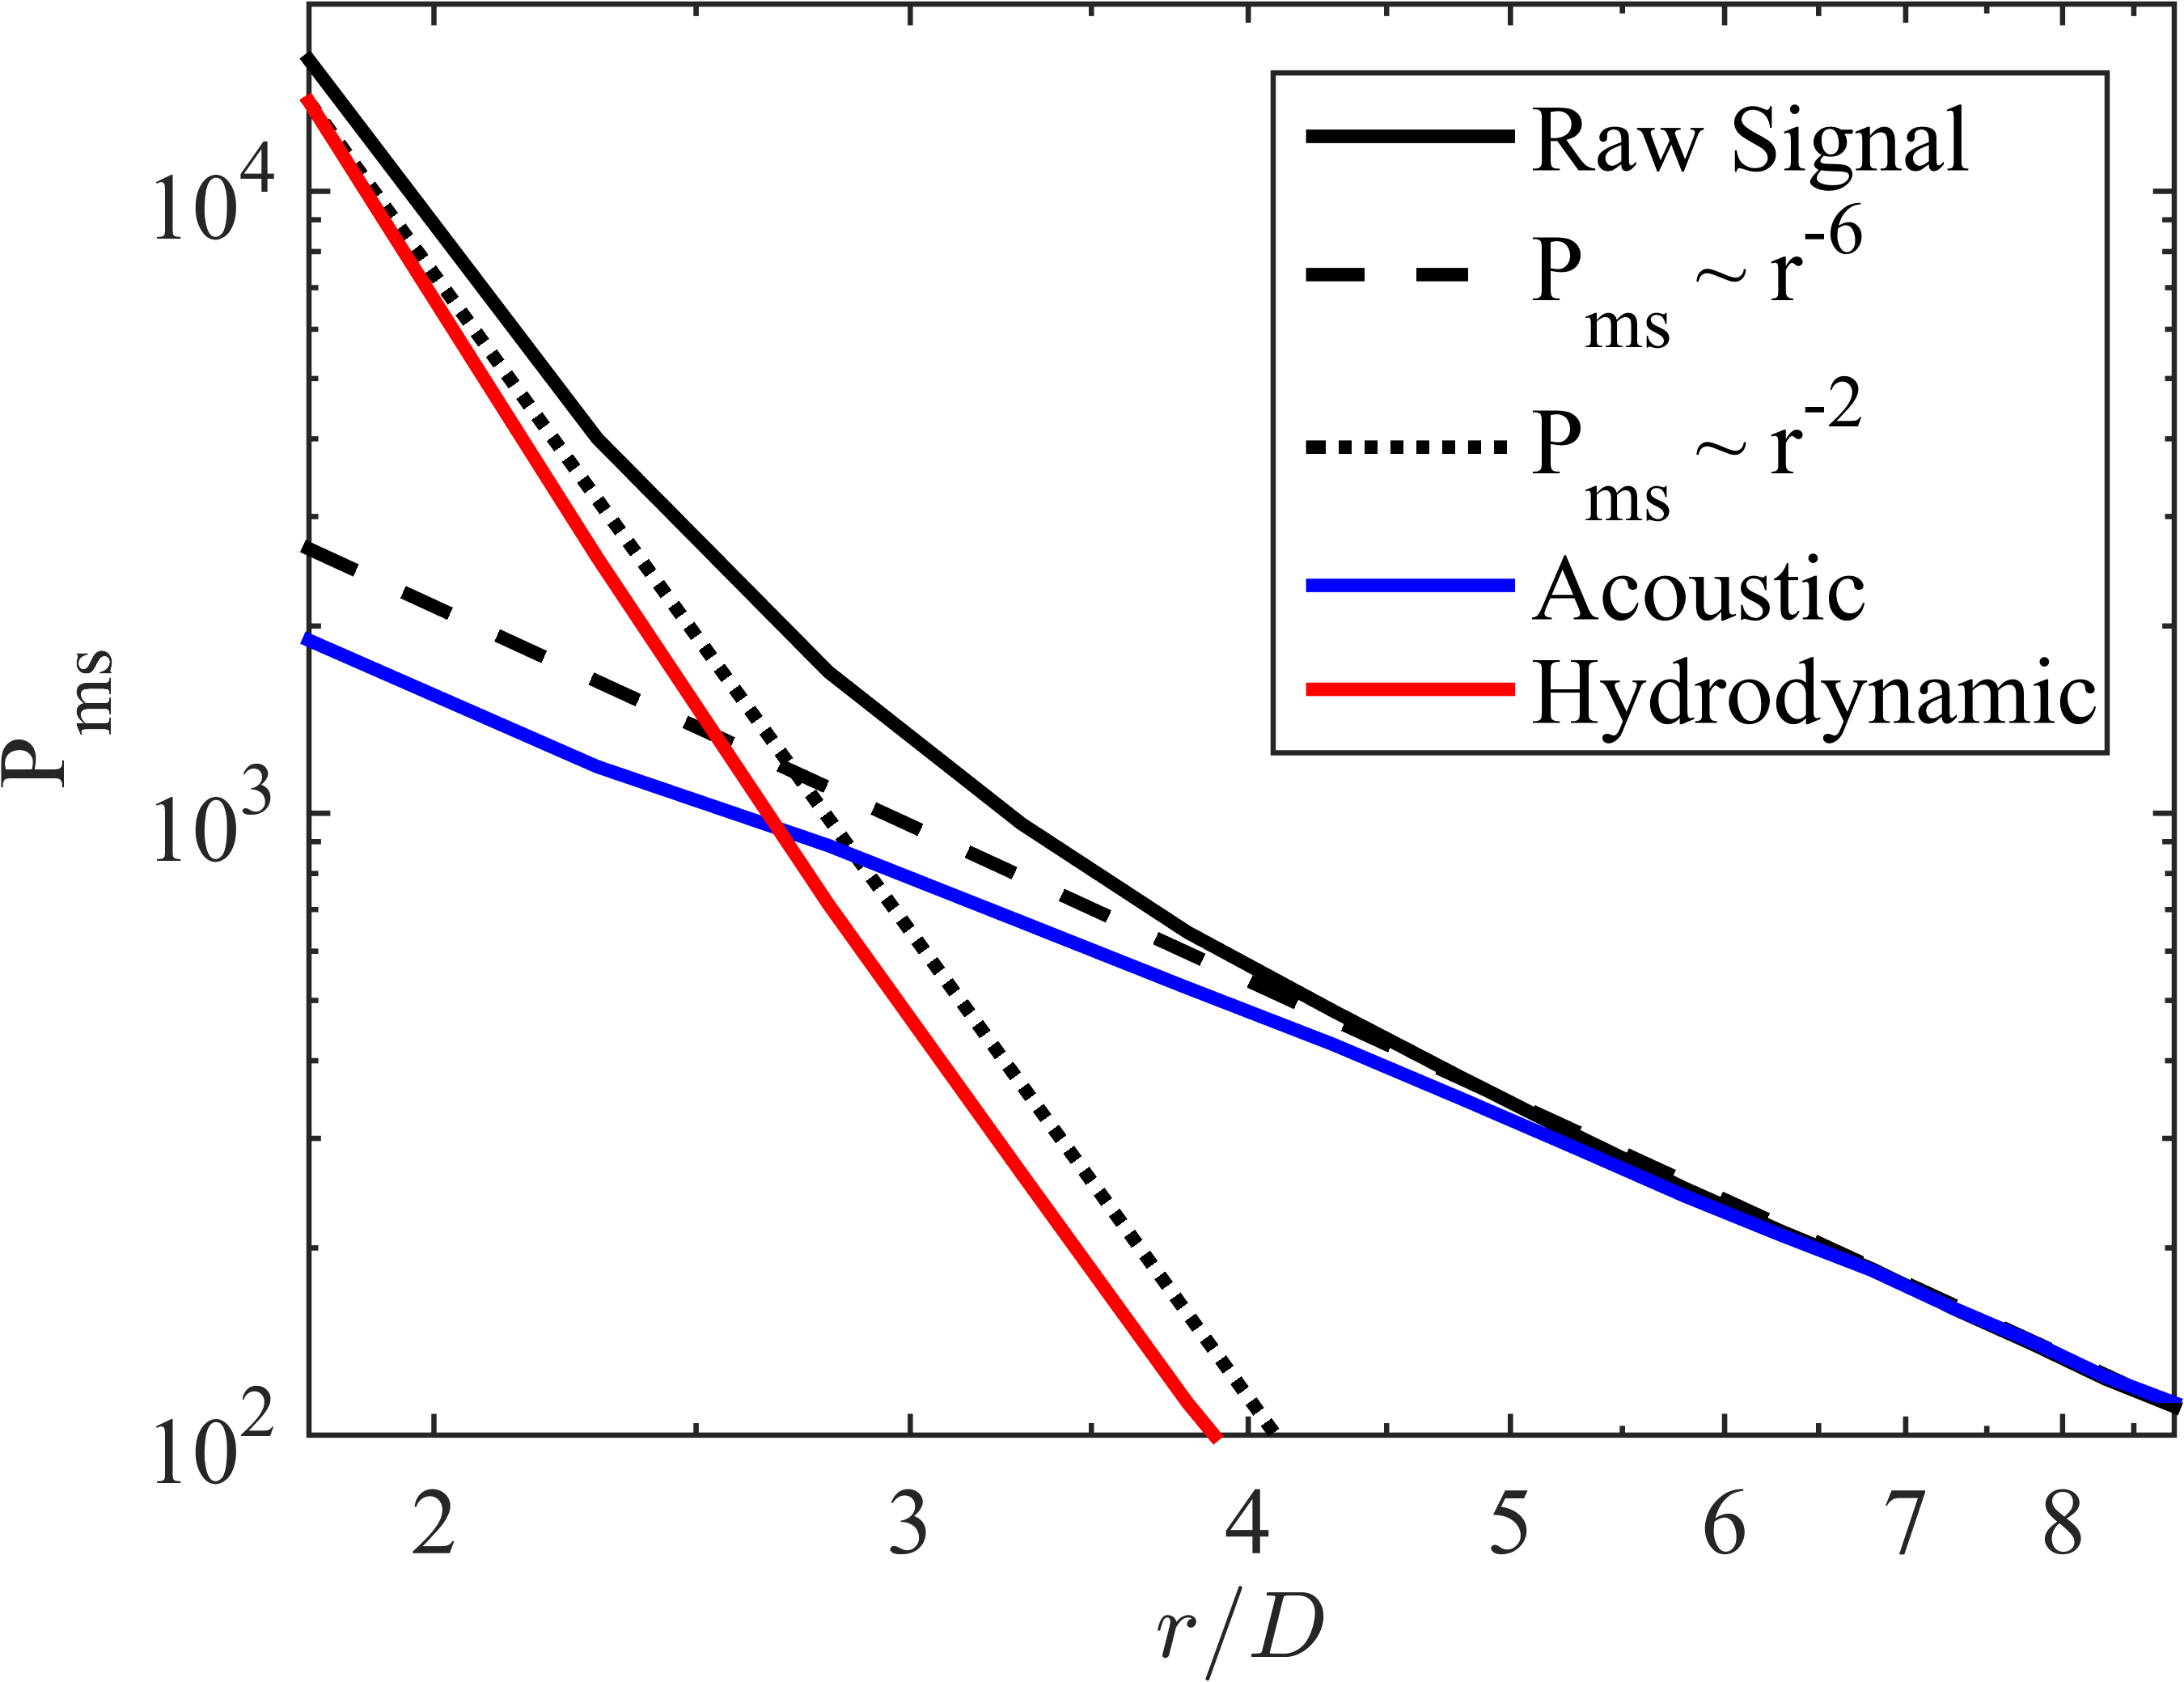
\includegraphics[width=4in]{Figures/ch3_validation_Pms.png}
	\caption{Radial decay of the raw signal compared against the theoretically-obtained and experimentally-measured decay rates for the acoustic and hydrodynamic components.}
	\label{fig:ch3_validation_Pms}
\end{figure}

Further insight into the veracity of the recovered acoustic and hydrodynamic fields may be obtained through analysis of the energy spectrum.
Like the radial decay rate of the pressure fluctuation intensities, Fourier analysis is inherently suited for random processes and hence has been shown to miss certain important aspects of the jet noise process (e.g.,  intermittency). 
However, it has been used extensively throughout the aeroacoustic community for understanding the composition of both near-field pressure fluctuations as well as the acoustic far-field, to great success. 
Fundamental models in jet turbulence and aeroacoustics (e.g. the spectral decomposition of the irrotational near-field by Arndt \etal [cite] and Tam’s similarity spectra for the acoustic far-field [cite]) analyze their respective phenomena in the Fourier domain.

Sample spectra taken at $z/D = 8, r/D = 2.2$ for the decomposed fields are shown in \fig{fig:ch3_validation_spectra}.
In the case of the hydrodynamic field (\fig{fig:ch3_validation_spectra_hydro}), the decomposed signal has be plotted against the raw near-field pressure spectrum as well as the $I \sim k^{-6.67}$ spectral decay rate in log space (with frequency/wavenumber) that was identified by Arndt \etal [cite] as the decay rate for the inertial subrange of the irrotational near-field.
As one would expect for positions just outside the jet shear layer, the decomposition has identified the dominant spectral energy of the near-field as being hydrodynamic; the decomposed hydrodynamic field accounts for nearly the entire energy of the raw signal at low frequencies.
Beginning at moderate frequencies ($St_D \simeq 0.15$) a divergence between the raw irrotational near-field and the decomposed hydrodynamic field is observed, due to the increasing relative intensity of the acoustic field.
At frequencies above this threshold, the decomposed hydrodynamic field exhibits a decay rate that matches quite well with the theoretical prediction, over several orders of magnitude. 

The decomposed acoustic spectrum acquired at this same near-field position is compared against the far-field acoustic signal simultaneously acquired at a polar angle of $30^\circ$ in \fig{fig:ch3_validation_spectra_acoustic}.
The acoustic spectrum has been scaled in amplitude in order to account for spherical propagation of the waves; calculating the propagation distances requires an assumption on the acoustic source region, which is not initially know with certainty.
As will be discussed in more detail in \sect{sect:near_field_source_region}, by measuring the time delay in two-point correlations between the near-field microphones and the far-field microphone at 30° the location of the dominant acoustic source region can be identified. 
In brief, the region just upstream of the end of the potential core ($z/D =4$) will be identified as the source region for the coherent large-scale structures in the jet; the current validation uses this location as the source region to scale the spectral amplitudes.
The signal at $z/D = 8, r/D = 2.2$ was chosen for this task as it lies roughly along a $30^\circ$ path from this assumed source region.
Additionally, the spectra were adjusted per ANSI S1.26 [cite] in order to account for atmospheric absorption of the (primarily high-frequency) acoustic waves due to propagation through a humid medium; the spectra shown here correspond to lossless propagation.
Lastly, the spectral peaks have been denoted by triangular markers at the top of the figure. 

It is found that the decomposed acoustic spectrum accurately reproduces the high-frequency portion of the far-field spectrum, which is unsurprising, given that the near-field spectra are dominated by acoustic fluctuations over this range of frequencies (though this does reinforce the accuracy of the amplitude-scaling used in the analysis).
Overall, the acoustic spectra extracted by the wavelet filter mirrors the far-field spectra quite well in terms of both spectral shape and amplitude, producing a `peaky' spectrum in contrast to the much more broadband raw irrotational near-field. 
The spectral peak occurs at nearly the same frequency as in the far-field, and is within 2 dB of the peak amplitude. 
The one major inaccuracy of the wavelet-based method is the failure to accurately reproduce the low-frequency spectral decay rate of the far-field spectrum. 
\begin{figure}
	\centering
	\begin{subfigure}{.5\textwidth}
		\centering
		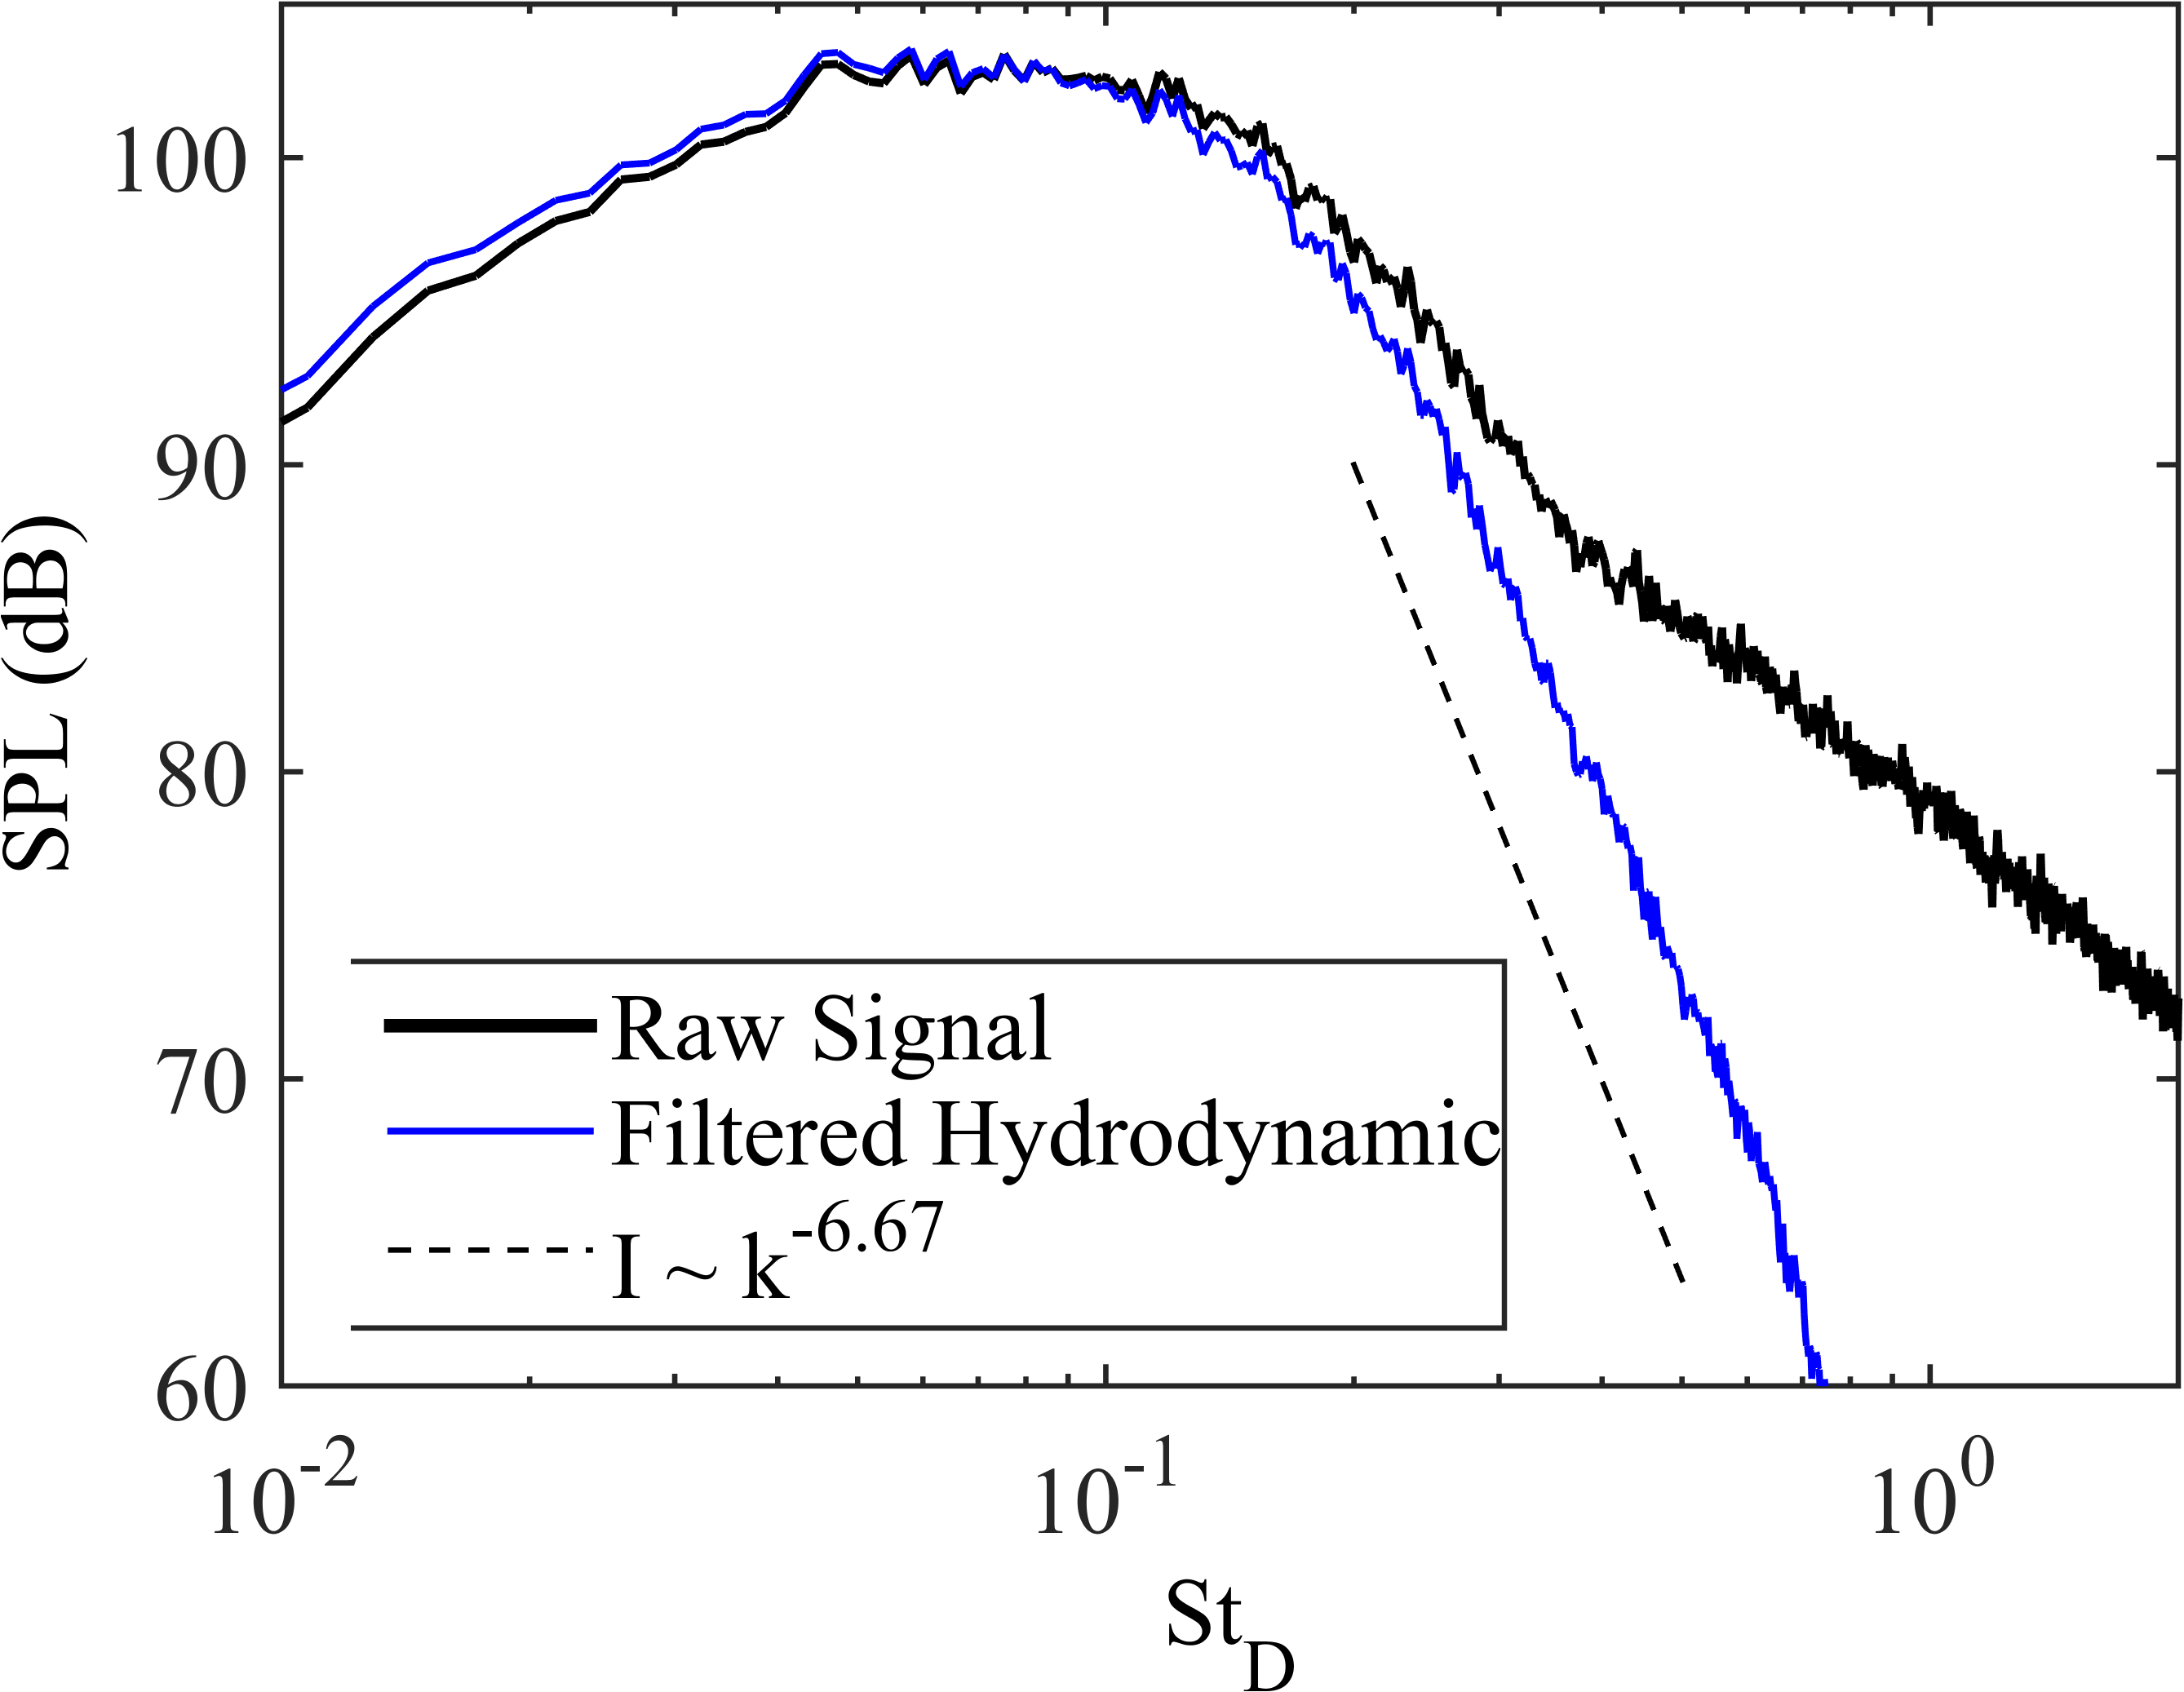
\includegraphics[width=0.95\linewidth]{Figures/ch3_validation_spectra_hydrodynamic}
		\caption{Hydrodynamic Decomposition}
		\label{fig:ch3_validation_spectra_hydro}
	\end{subfigure}%
	\begin{subfigure}{.5\textwidth}
		\centering
		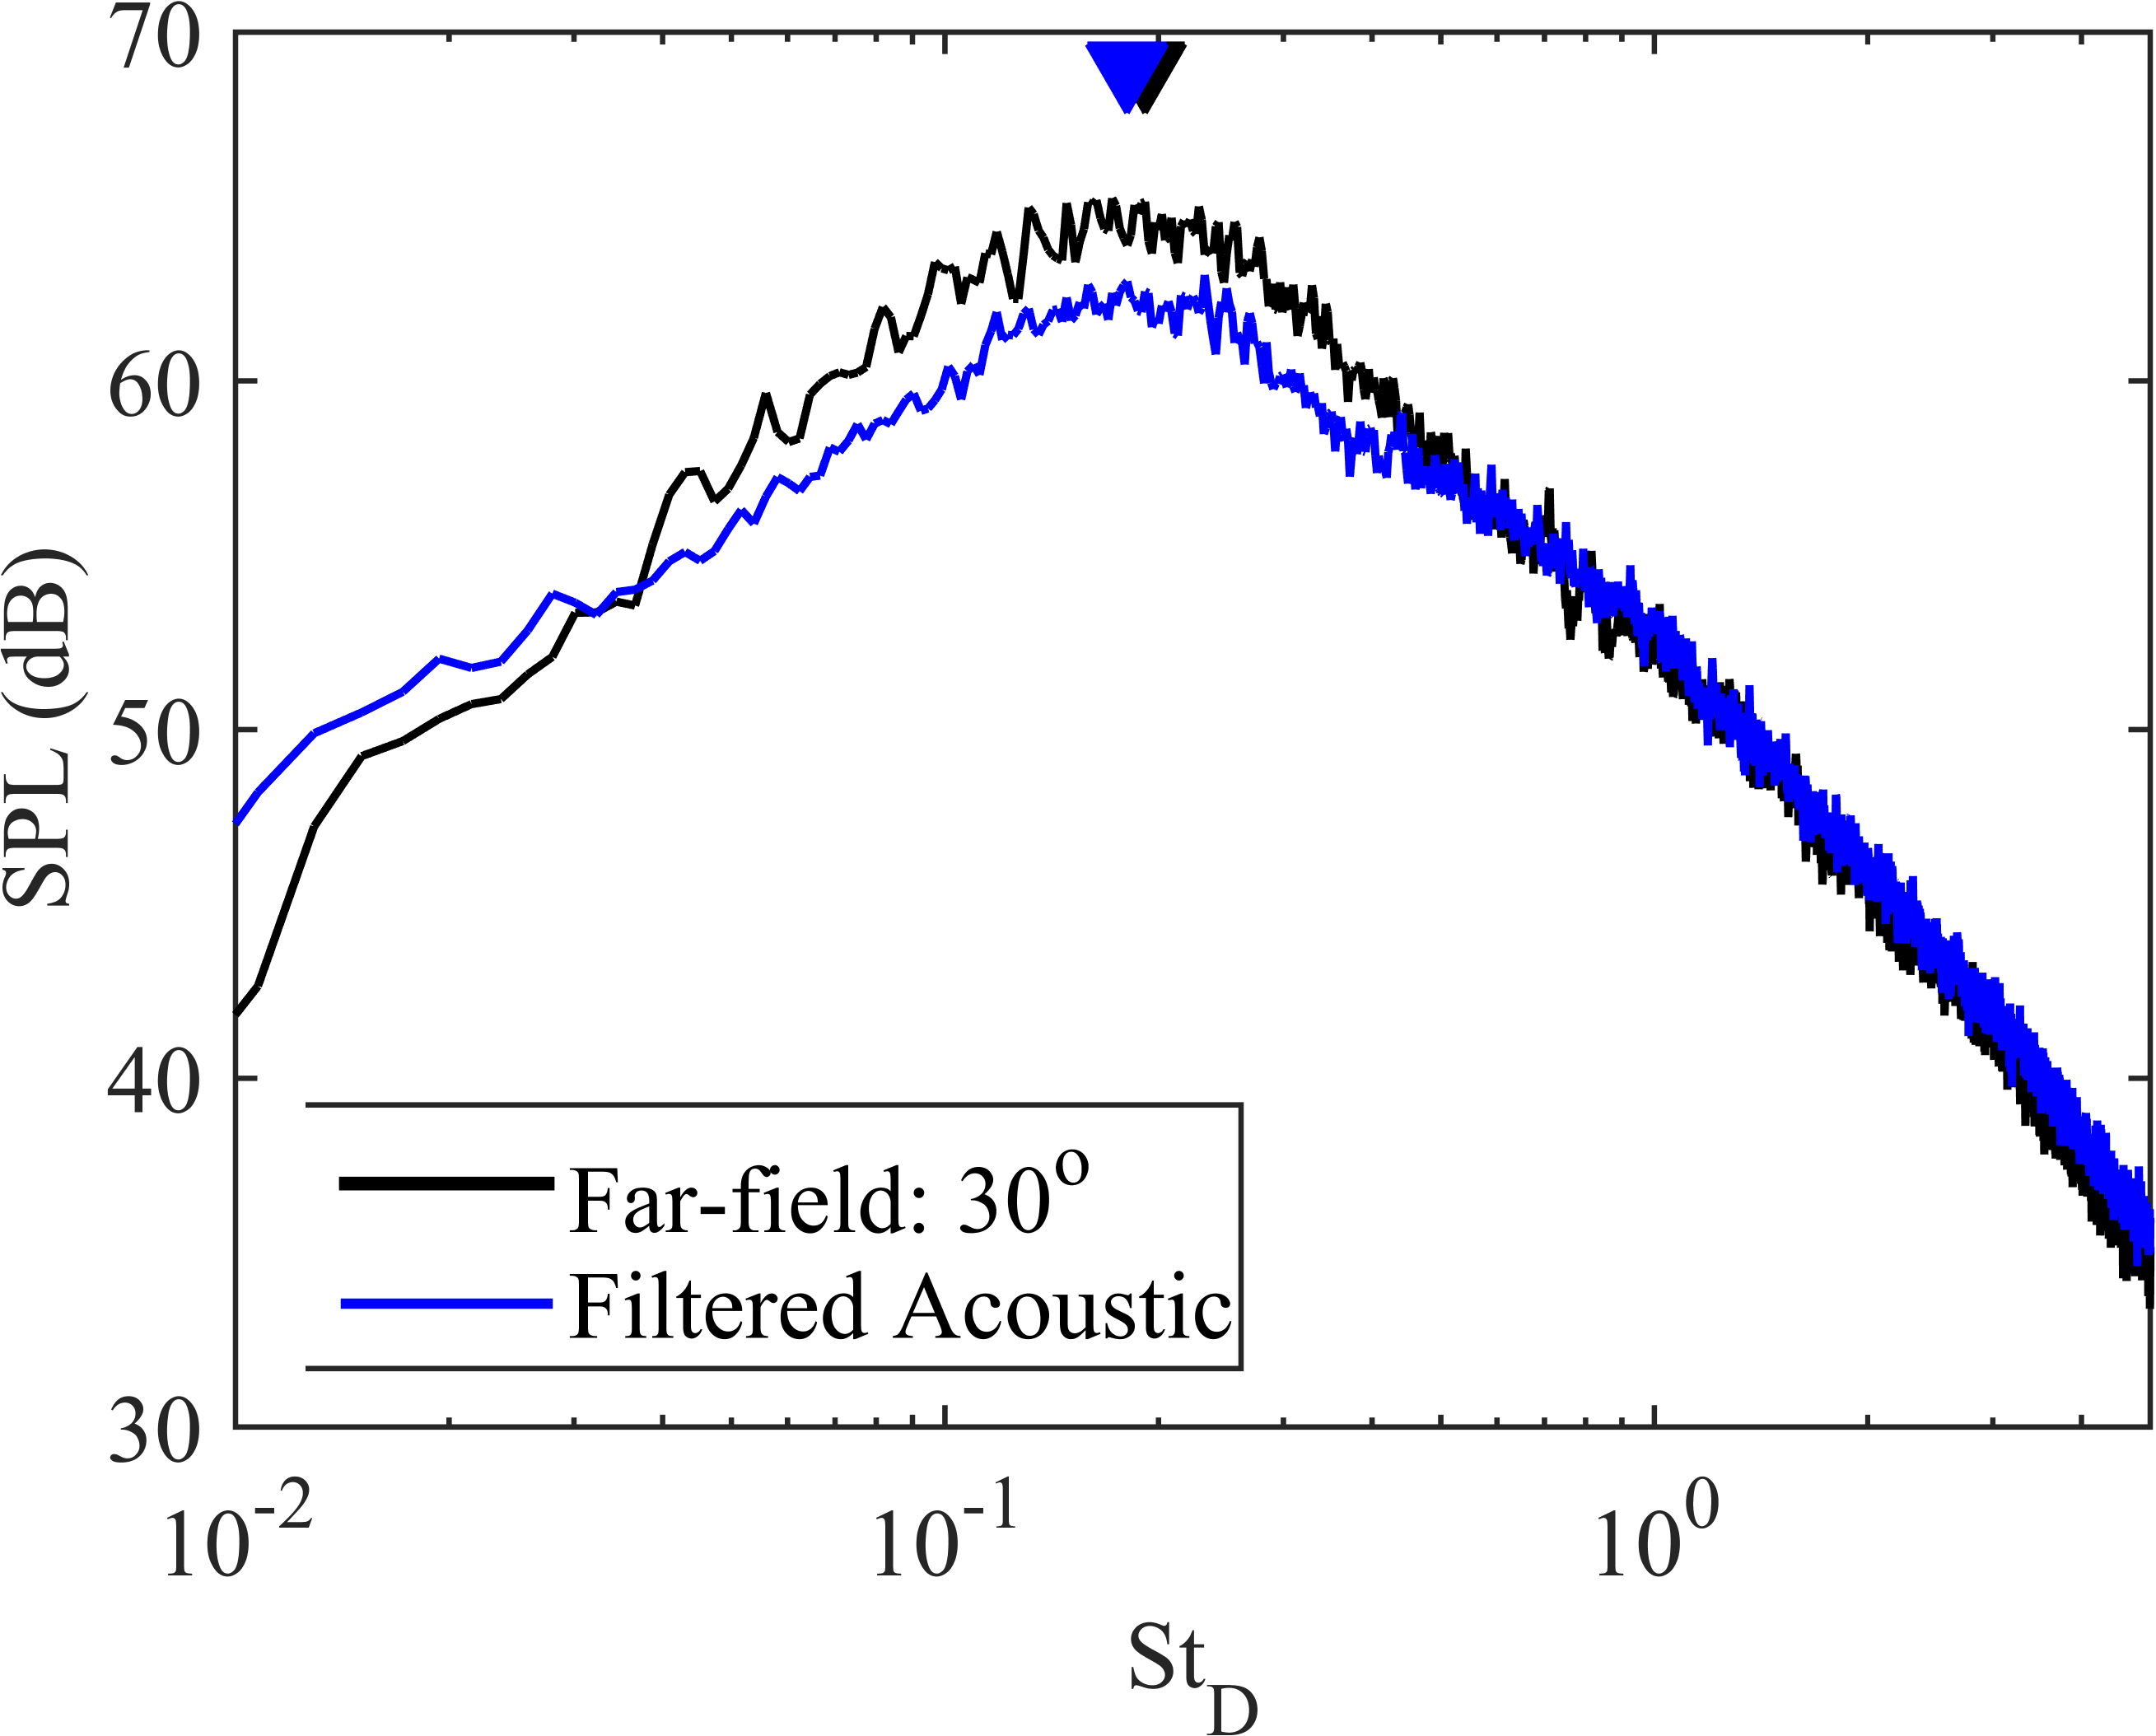
\includegraphics[width=0.95\linewidth]{Figures/ch3_validation_spectra_acoustic}
		\caption{Acoustic Decomposition}
		\label{fig:ch3_validation_spectra_acoustic}
	\end{subfigure}
	\caption{Spectral comparison of decomposed hydrodynamic field compared against the raw near-field signal (a) and decomposed acoustic field compared against the far-field acoustic signal at $30^\circ$. In both cases, the near-field signal was acquired at $z/D = 8, r/D = 2.2$}
	\label{fig:ch3_validation_spectra}
\end{figure}

As a final method of validation, the decomposed fields for the excited jet were analyzed in the time domain by phase-averaging.
As has been pointed out by numerous other researchers [Cavalieri, Camussi, Kearney-Fischer, Hileman], the turbulent jet and resultant acoustic field are highly intermittent phenomena. 
An illustration of this behavior can be found in \fig{fig:ch3_wavelet_spectrum}, where the wavelet power spectrum of the far-field at $30^\circ$ has been plotted as a function of (pseudo) Strouhal number and time for the unforced jet; this can be compared against the Fourier power spectrum presented in \fig{fig:ch3_validation_spectra_acoustic}. 
As with the Fourier analysis, wavelet analysis demonstrates that the baseline jet radiates to the far-field over a broad range of Strouhal numbers, with the dominant energy occurring for $St_{DF} \simeq 0.15$. 
However, the far-field is found to be composed of temporally- and frequency-localized bursts of energy – far from the stationary field that Fourier analysis assumes. 
Clearly, this intermittent behavior needs to be recovered in the near-field by the decomposition process; something which may be evaluated with the aid of LAFPA excitation.
\begin{figure}
	\centering
	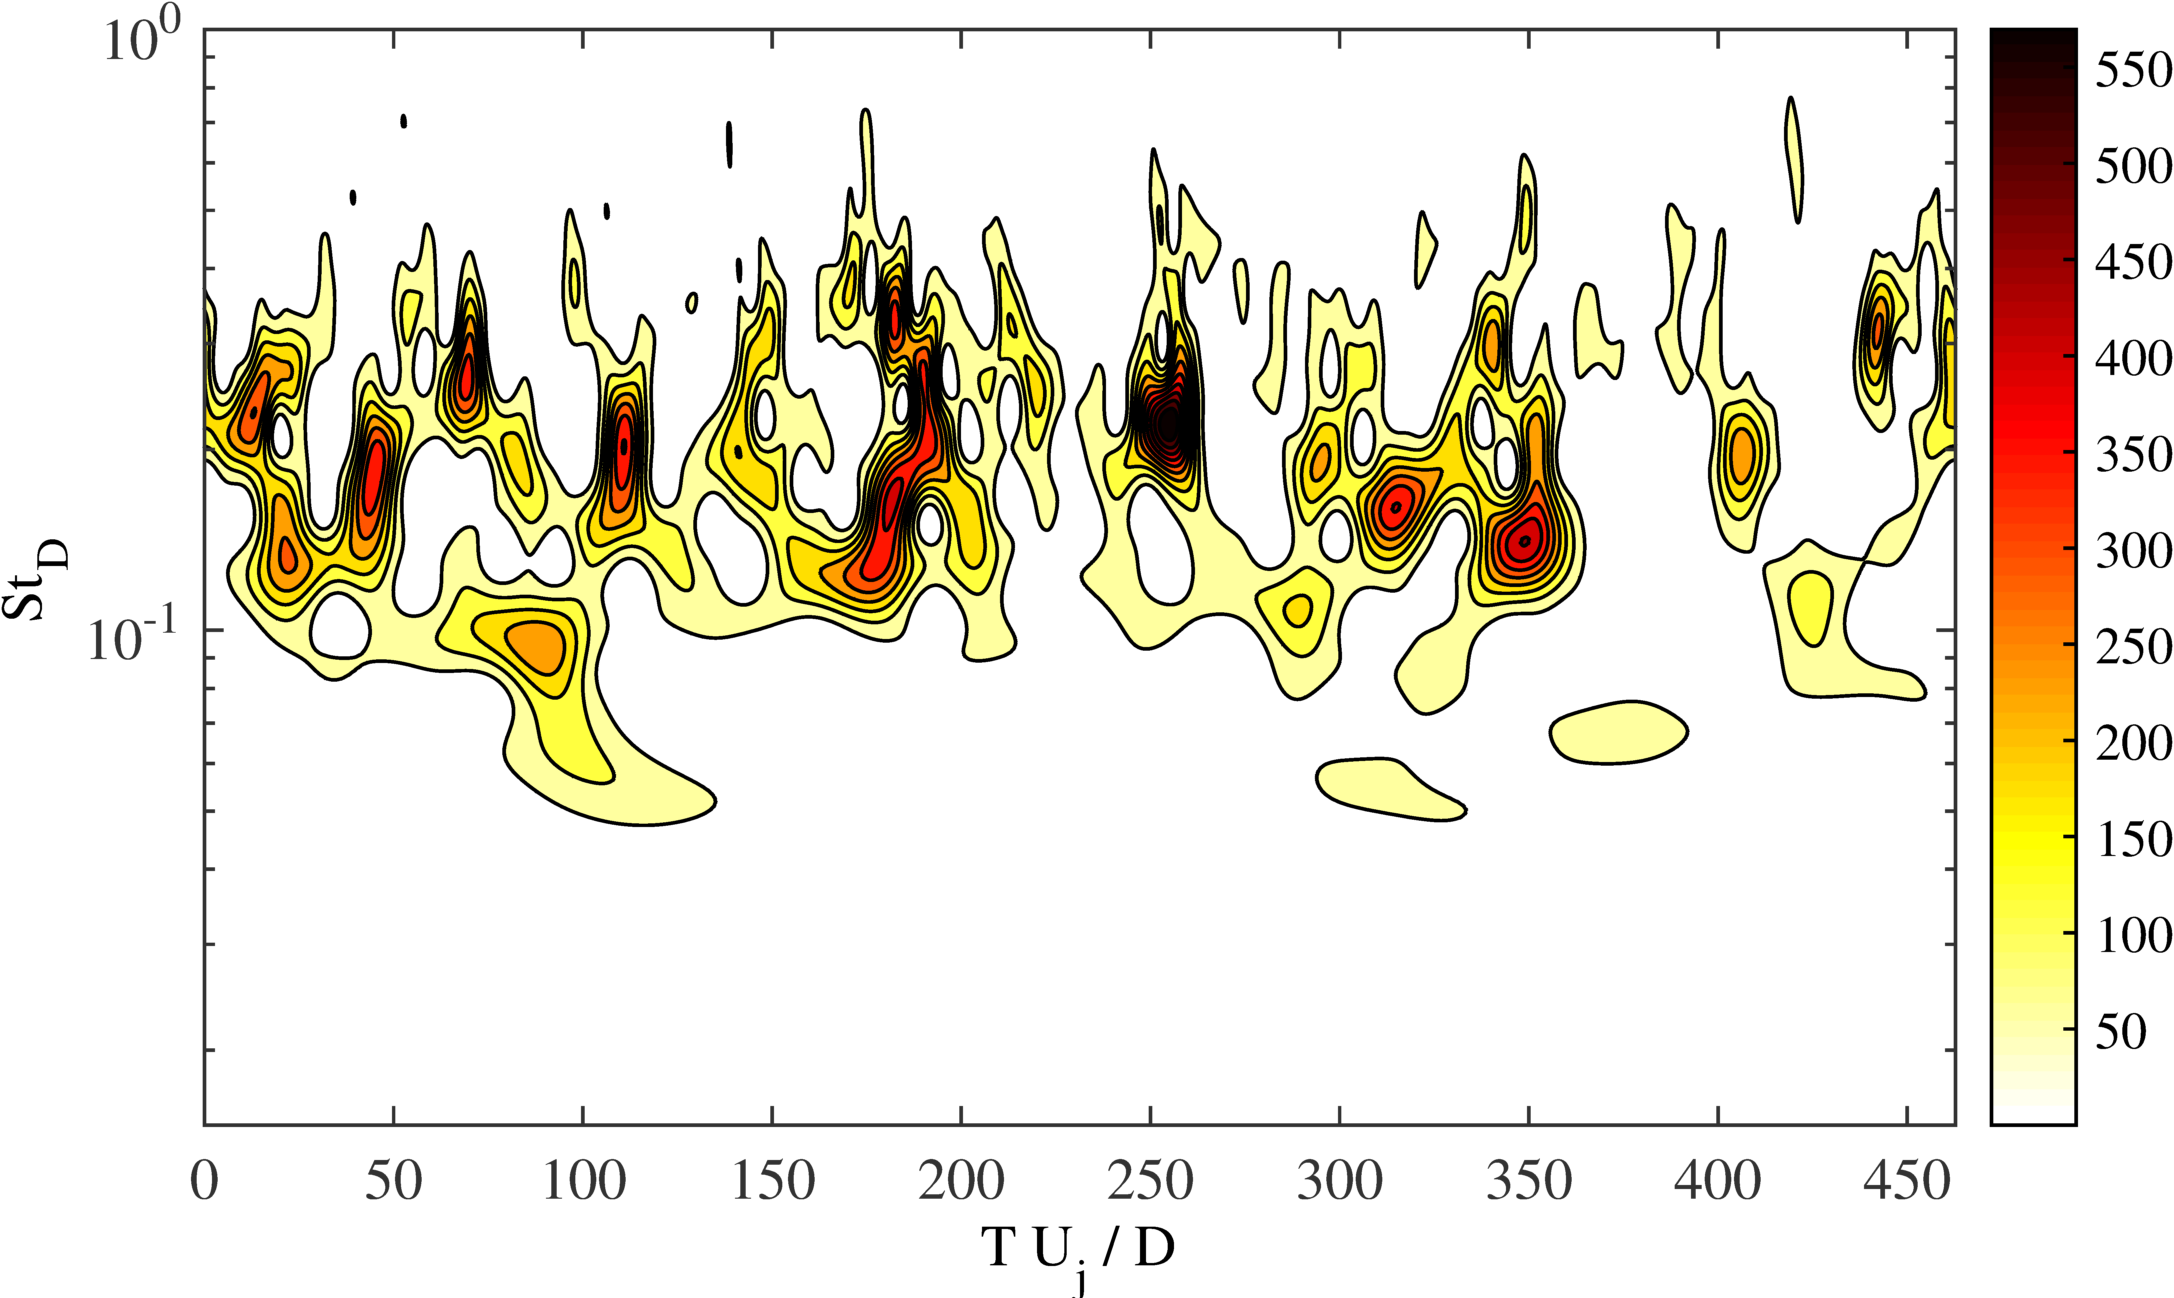
\includegraphics[width=4in]{Figures/ch3_wavelet_spectrum.png}
	\caption{Wavelet power spectrum in the acoustic far-field at $30^\circ$ for the unforced jet.}
	\label{fig:ch3_wavelet_spectrum}
\end{figure}

As before, the decomposed acoustic signal at $z/D = 8, r/D = 2.2$ was propagated to the far-field at $30^\circ$ by scaling the amplitude according to $I \sim r^{-2}$; the phase-averaged signal was also shifted in time based on the ambient speed of sound in order to account for the propagation delay. 
Results of this procedure can be found in \fig{fig:ch3_validation_phavg} for the jet excited at $St_{DF} = 0.05$. 
For illustrative purposes, results computed using the more standard Fourier-based decomposition method have also been included here.
Both the Fourier and wavelet methods identify a distinct waveform which matches quite well with the waveform observed in the far-field, though with some discrepancies. 
The wavelet-method produces a slightly more accurate peak amplitude and event temporal extent. 
The most significant difference between Fourier and wavelet methods is the existence of severe ringing (caused by Gibbs’ phenomena) observed in the Fourier results just preceding the acoustic event. 
This phenomena persists even when the events are no longer strictly intermittent, (not shown here for brevity). 
\begin{figure}
	\centering
	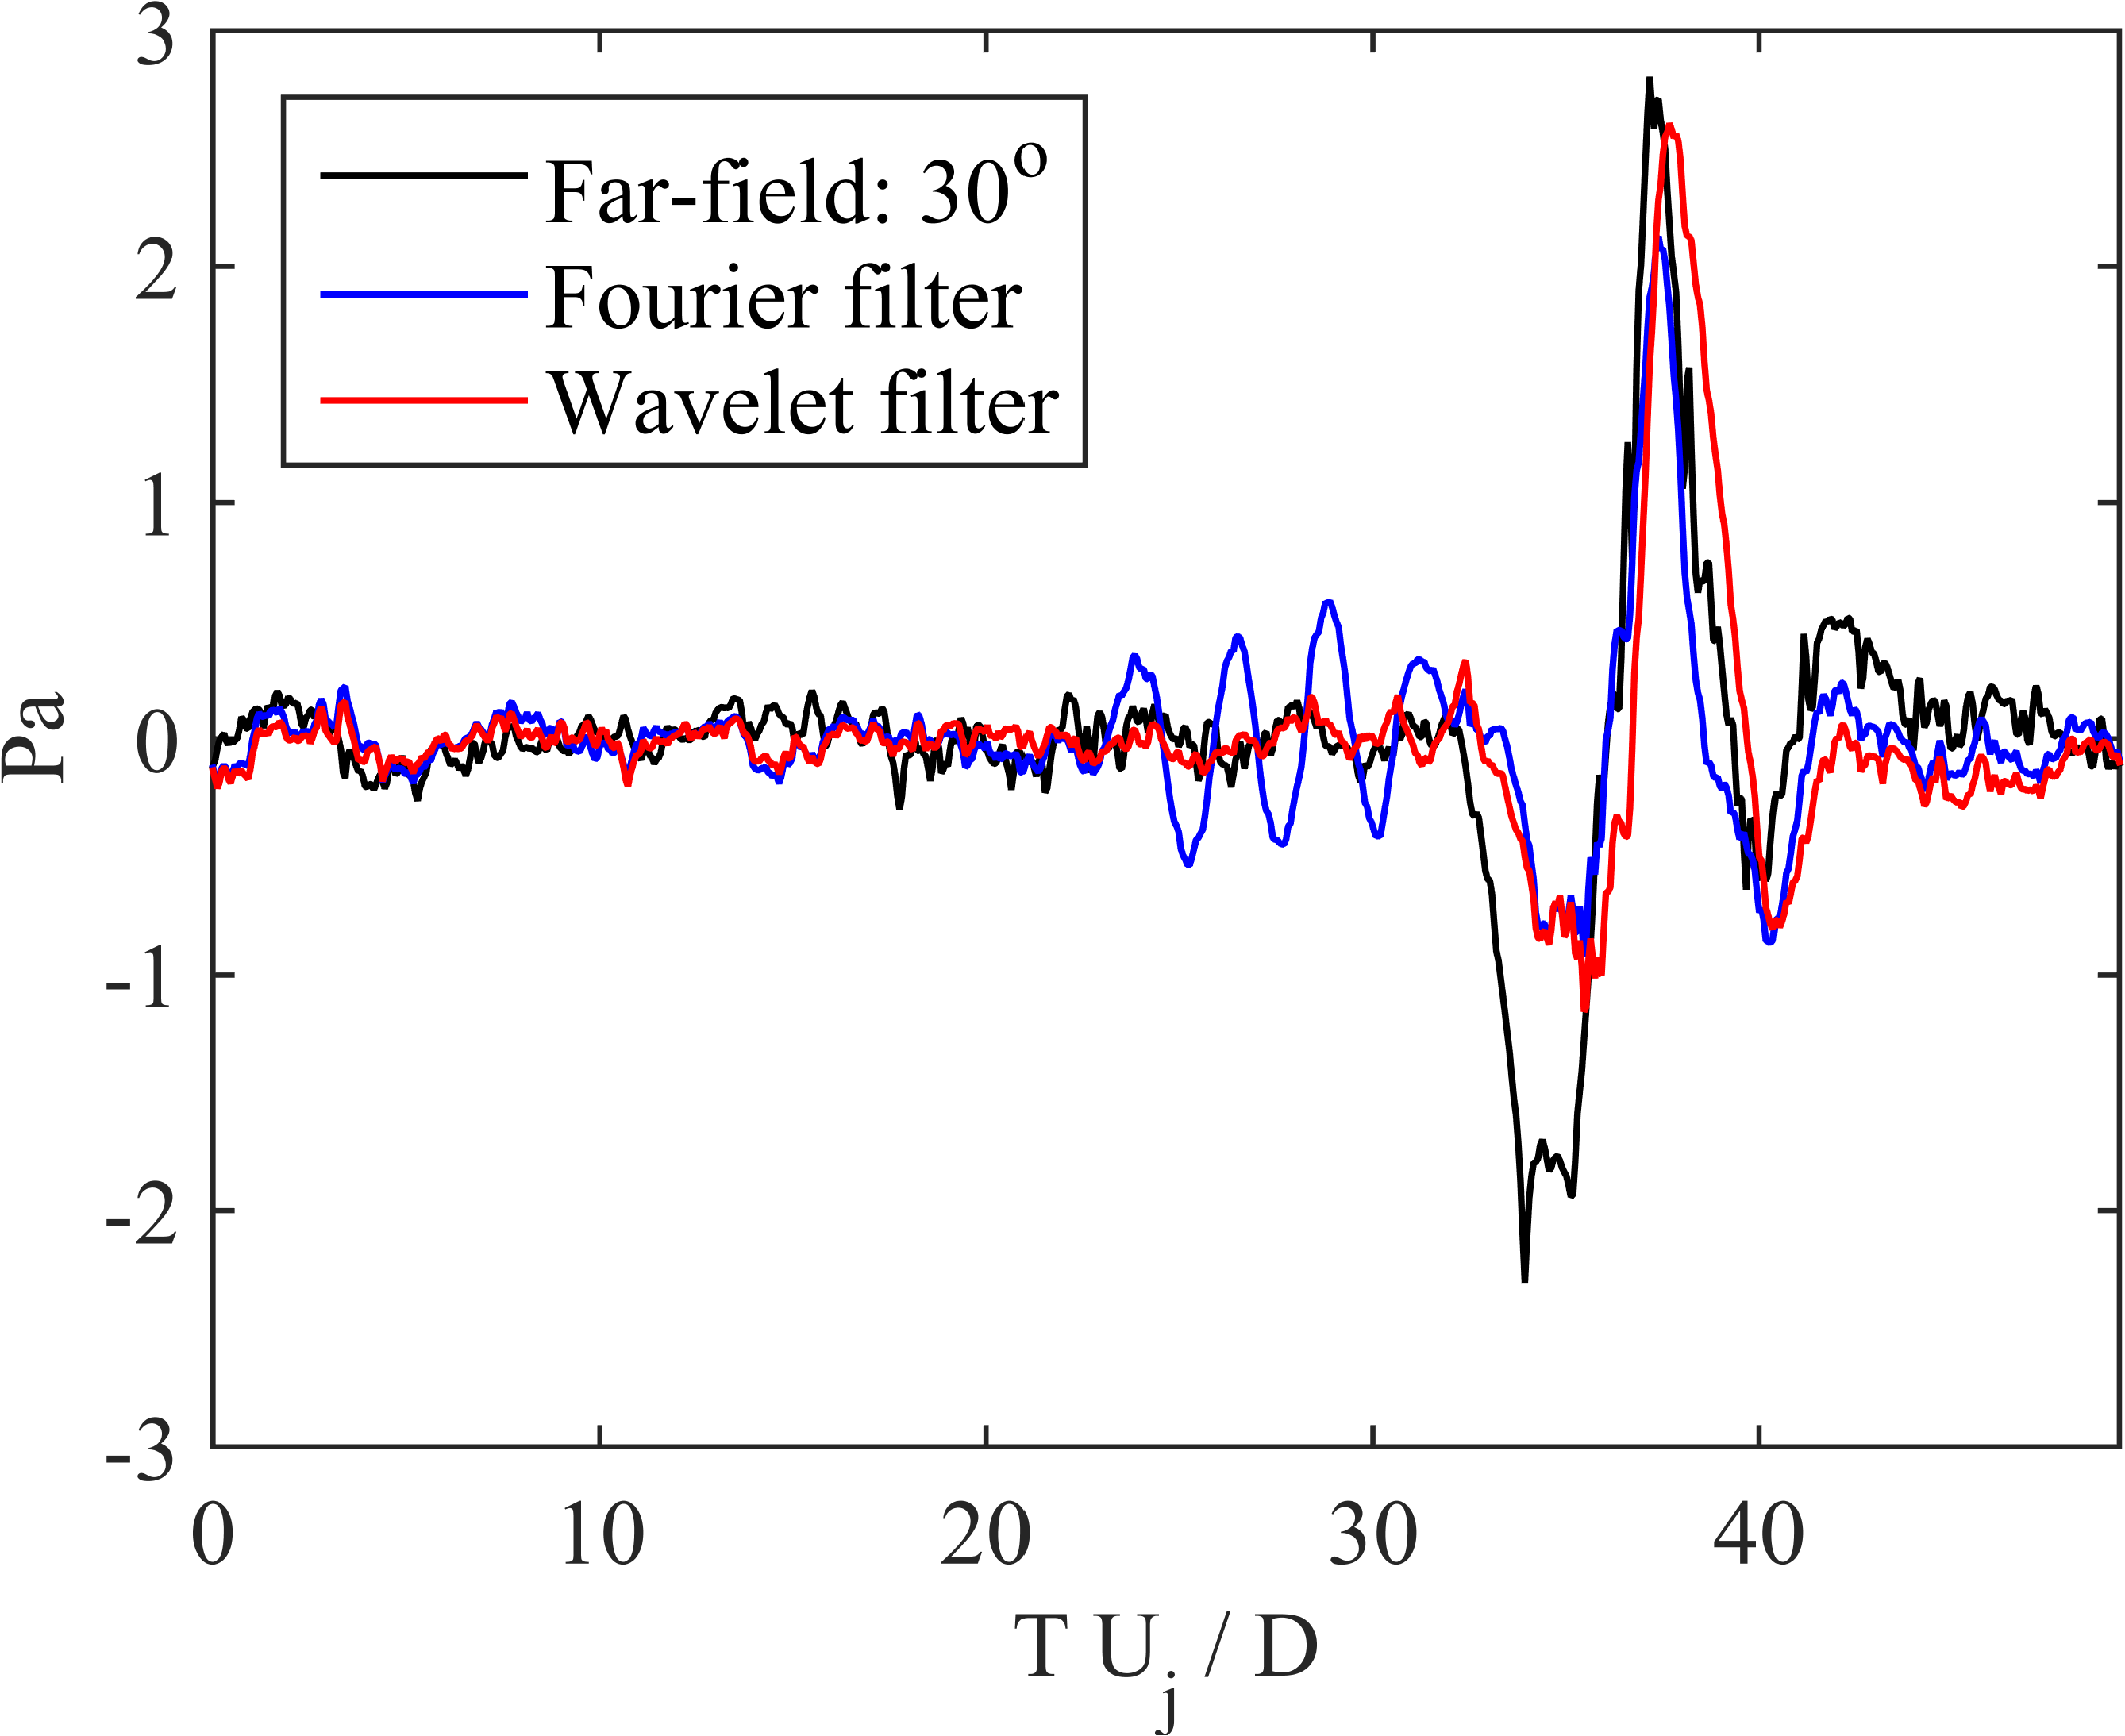
\includegraphics[width=4in]{Figures/ch3_validation_phavg.png}
	\caption{Comparison of phase-averaged waveforms produced by excitation at $St_{DF} = 0.05$. As before, the near-field signal was acquired at $z/D = 8, r/D = 2.2$}
	\label{fig:ch3_validation_phavg}
\end{figure}

In the case of a subsonically-convecting jet, the conceptual basis behind the Fourier decomposition algorithm is not in error (excluding the periodicity assumed by the Fourier transform). 
Instead, the practical requirements of discretely sampled microphones spanning a finite region in space, in addition to noise in the data acquisition, lead to numerical artifacts in the reconstructions. 
The Fourier transform required an extensive axial array of microphones (16 microphones spanning $21D$ in the current study) in order to accurately represent the pressure fluctuations (the array was originally designed with the intent of using the  Fourier-based decomposition).  
This is because the basis functions (trigonometric function) used in the Fourier transform are not physically representative of the physical phenomena under study. 
As discussed previously, the turbulent jet (and resultant acoustic field) is highly intermittent. 
Even with the excitation producing regular large-scale structures, these, as well as the resultant acoustic emissions, exist as temporally and spatially localized energy bursts, rather that space-filling sinusoidal waves (as assumed by the Fourier transform). 
It has been shown that by using a temporally/spatially localized fluctuation as a basis, the wavelet transform compresses the information in a turbulent field much more efficiently (and accurately) than the Fourier transform [Farge].

Though there are some relatively minor discrepancies between the expected acoustic near-field and the one produced by the spatio-temporal wavelet filter, overall the results are promising.
The decomposition algorithm is extracting hydrodynamic and acoustic fields which accurately reproduce the expected radial and frequency decay rates per theoretical analysis over the large domain investigated in this work (both in terms of spatial and frequency/wavenumber extent).
Additionally, this accuracy is also not just a statistical phenomenon, as the decomposition algorithm is also found to accurately identify and reconstruct strongly-energetic, localized bursts of energy in the constitutive fields. 
Based on these results, the author felt confident that the decomposed acoustic field produced by the spatio-temporal wavelet filter was highly representative of the true acoustic near-field.

\section{Identifying the Acoustic Source Region}
\section{Hydrodynamic Wavepackets}
\label{sect:near_field_source_region}